\subsection{Syntax-number units interactions}

\begin{figure*}[t]
    \centering
    \begin{subfigure}{0.49\textwidth}
            \centering
            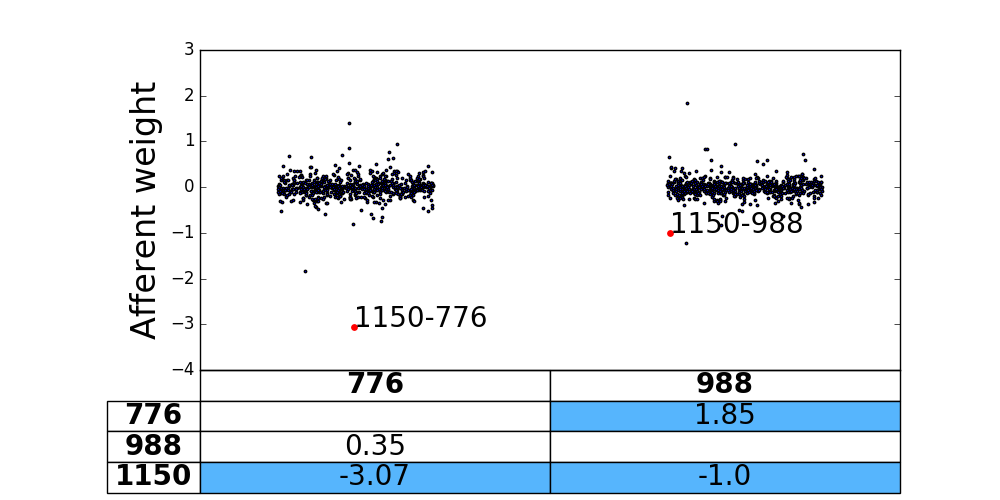
\includegraphics[width=\textwidth]{Figures/gate_Input_afferent_interactions.png}
            \caption{Input gate}
            \label{fig:interaction-input}
    \end{subfigure}
    \begin{subfigure}{0.49\textwidth}
           \centering
          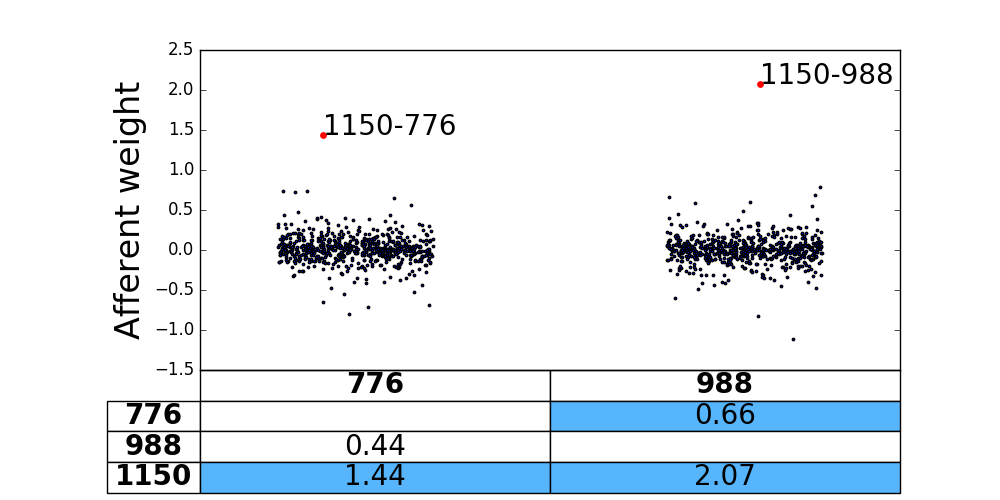
\includegraphics[width=\textwidth]{Figures/gate_Forget_afferent_interactions.png}
          \caption{Forget gate}
          \label{fig:interaction-forget}
    \end{subfigure}
\caption{Connectivity among the syntax and two LR-number units.}
\label{fig:interaction}
\end{figure*}

The previous sections described two crucial factors required to solve the NA-task by the network - units that encode and carry the subject number across long-range dependencies, and a unit that encodes the main subject-verb dependency. We now look into the interactions among these units by analyzing the weights in the network. We note that for each pair of units there are four types of connections corresponding to the four types of gates in the units. Each type of weight can thus contribute to a different type of interaction, depending on the function of the gate. 

Figures \ref{fig:interaction-input} and \ref{fig:interaction-forget} present the distributions of all afferent recurrent weights to the singular and plural units, for the input and forget gates. Weights from the syntax units are marked in red and are labeled. Table values represent weight sizes among the units (projecting units appear to the left of the table), and blue background represents significance of the corresponding weight size compared to all other weights ($p-value<0.05$). Results show that the weights from the syntax unit to the forget gate of both number units are exceptionally high compared to all other afferent connections in the network (rank, $p-value=$,), and exceptionally low to their input gates (rank, $p-value$). 

Since cell activity of the syntax unit is positive across the entire subject-verb dependency (e.g., figure \ref{fig:syntax-unit-double-subjrel}), the connectivity from the syntax unit drives the forget gate of the number units towards a value of one ($W^f_{776, 1150}h_{1150}>0$) and their input gates towards a value of zero ($W^i_{776, 1150}h_{1150}<0$). Looking at the r.h.s. of equation 1, this means that the first term becomes dominant and the second term goes to zero, suggesting that across the entire dependency the syntax unit conveys a \textit{'remembering signal'} to the number units, and, similarly, when the activity of the syntax unit becomes negative, the syntax unit conveys an \textit{'update signal'} to them both at the end of the dependency. 

Last, we note that the weight values between the two LR-number units are significantly high compared to all other afferent connections. Since their activity of both units is negative across the dependency (Figure \ref{fig:singular-unit} and \ref{fig:plural-unit}), this means that they are \textit{mutually inhibiting}, thus warranting an unequivocal signal about the grammatical number of the subject to the output layer.

